\documentclass{article}
\usepackage[a4paper, top=2cm, bottom=2cm, left=2.5cm, right=2.5cm]{geometry}
\usepackage{graphicx}
\usepackage{float}
\usepackage{amsfonts}
\usepackage{amsmath}
\usepackage{listings}
\usepackage{xcolor}
\usepackage{hyperref}
\usepackage[dvipsnames]{xcolor}
\usepackage[normalem]{ulem}

% Titolo
\title{Appunti sistemi embedded}
\author{Federico Falcone}
\date{\today}


\begin{document}

\maketitle
\tableofcontents
\newpage

sketch->programma \\
no protezione memoria

\section{Elettricità}
Elettricità composta da elettroni che scorrono. Essi scorrono se il materiale lo permette. Applicando una forza elettrica l conduttore gli elettroni si spostano.
La forza applicata per spostare gli elettroni si chiama \textcolor{red}{tensione} (V). La tensione è la forza con cui io tiro o spingo gli eletrtoni negli elettroni. Tanto è più la forza la velocità non aumenta o diminuisce. Ciò che succede è che aumenta la quantità
di elettroni che scorrono. La quantit di elettroni che si muovono nella quantità di tempo si chiama \textcolor{red}{intensità} (A, ovvero Coulomb per secondo). Quindi aumentando la tensione aumenta l'intensità.
La legge che regola la variazione del flusso di corrente rispetto alla forza che io applico è la legge di Ohm e coinvolge un terzo parametro che dice quanto è gnucco il conduttore nel reagire all'applicazione della forza.
\\ Anche se non è vero, si definisce un conduttore ciò che ha resistenza 0 (in realtà e bassissima). Tutto ciò che oppone resistenza sostanziale, si chiama \textcolor{red}{resistenza}.
\\ La legge di Ohm ci permette di calcolare uno dei 3 parametri conoscendone 2.
La resistenza dipende anche dalla dimensione del conduttore.
\\\textbf{Legge di Ohm}:$V=R \cdot I $\\
\textbf{Potenza}\\
La potenza ci dice quanto lavoro posso fare con un certo apparato, o quanta energia sta consumando in un dato istante, o quanto può durare un batteria. ci permette di capire quanto è "forte", quanto è capace di fare operazioni importanti.
Si misuta in Watt (W)
\[ P=V \cdot I \]
La resistenza nell'opporsi agli elettroni, fa un lavoro, e quindi oppenendosi alla tensione brucia quel lavoro in calore . Trasforma il lavoro che ha fatto la tensione.
\\ La corrente gira in un circuito, se c'è un'interruzione si parla di \textcolor{red}{circuito aperto} (la corrente non circola). Nonostante ciò la corrente continua a fluire (perchè non esiste un isolante che isoli COMPLETAMENTE).
\\ La batteria è carica o scarica si miscura o gli Ah. Ampere ora permette di capire quanto la batteria è in grado di erogare id corrente nel tempo.
\\ Per capire la carica della batteria si può misurare la tensione, o misurando la potenza erogata dalla batteria. Per misurarla bisogna tirargli fuori la corrente tramite un consumatore che gli tira fuori più corrente possibile. Per fare ciò la resistenza deve essere più vicino allo zero possibile, creando così un
quasi corto circuito. Cosa io attacco per testare il suo carico serve a testare se riesce a gestire questo carico. \textbf{Problemi}: il carico massimo è molto diffiche da misurare, cortocircuitare crea calore (e  quindi si incendia). Per misurare in sicurezza si può, ma non misura comunque la potenza massima.
\\ Qualunque oggetto che assorbe potenza elettrica è un carico.
\\ Un meccanismo di protezione per evitare che un carico assorba più potenza di quella che può gestire è il fusibile. Esso si brucia se la potenza assorbita è troppo alta, interrompendo così il circuito e proteggendo il carico. (Oggi si usano i magnetotermici, che invece di bruciarsi, si staccano, e possono essere riattaccati una volta risolto il problema).
\pagebreak
\paragraph{Lezione 4} \mbox{}
\begin{figure}[H]
    \centering
    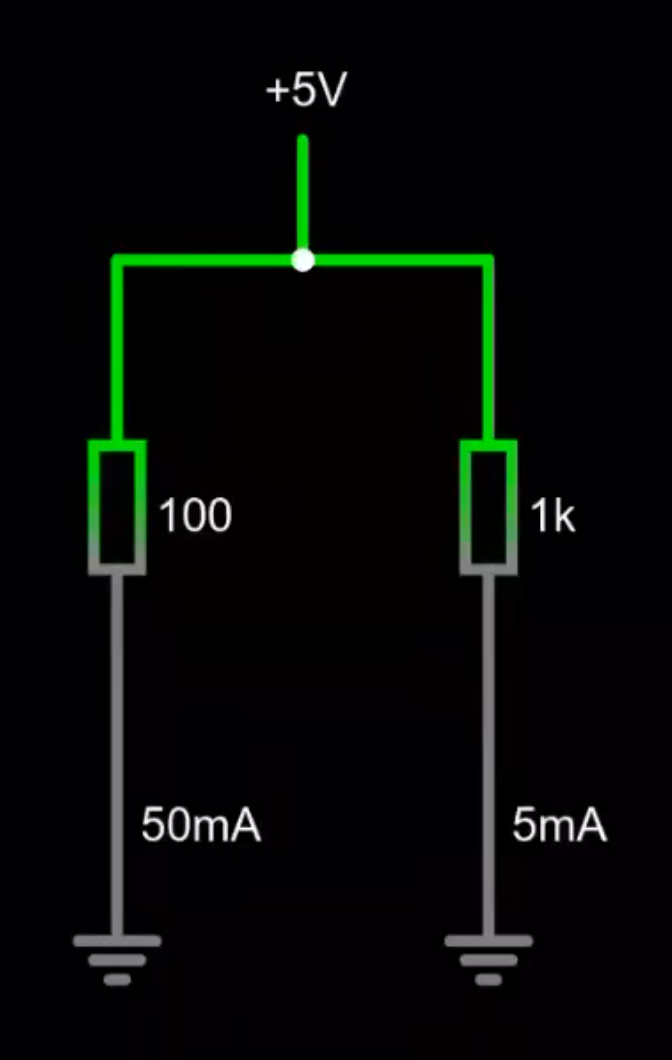
\includegraphics[width=0.25\textwidth]{Images/circuito1.png}
\end{figure}
Quando misuro una tensione, misuro un'energia potenziale. Quando io misuro in un punto è come se misurassi l'altezza/inclinazione di un piano inclinato. In quel punto ottengo qualche tipo di effetto. Il \textbf{groud} (terra) è come il piano nel piano inclinato. Tutto ciò che sta sopra al ground è una tensione utilizzabile. Una resistenza è come un piano inclinato e tanto più quella resistenza è bassa,
tanto più posso estrarre lavoro. Se metto una resistenza molto bassa, è come mettere un piano molto inclinato e quindi la biglia rotola molto velocemente. Al contrario la biglia rotola più lentamente.
\\ Nel momento in cui metto una resistenza, sto mettendo un piano inclinato. Nonostante le resistenze, il numero di elettroni che passano è sempre lo stesso.
\\ Attaccando delle resistenze in serie, è possibile ridimensionarla in un'unica resistenza. La corrente che passa è la combinazione di tutti gli effetti di strozzatura delle resistenze. Mettendo le resistenze in serie serve nel momento in cui abbiamo bisogno di una resistenza con un valore in particolare, ma che non esiste in commercio.
\\ In caso volessimo sapere la \textbf{quota} (tensione) all'uscita di una resistenza.
\\ Quando una corrente passa per una resistenza, si ha una \textbf{caduta di tensione}, ovvero la tensione si riduce. In altre parole la caduta di tensione è la tensione che devo applicare alla resistenza per farci passare esattamente una corrente.
\subsection{Prima legge di Kirchhoff}
La somma delle tensioni in un circuito fa 0.
\[ \sum_{i=1}^n V_i = 0 \]
La somma delle correnti di un nodo è 0.
\[ \sum_{i=1}^n I_i = 0 \]
\subsection{Connessione in parallelo}
\begin{figure}[H]
    \centering
    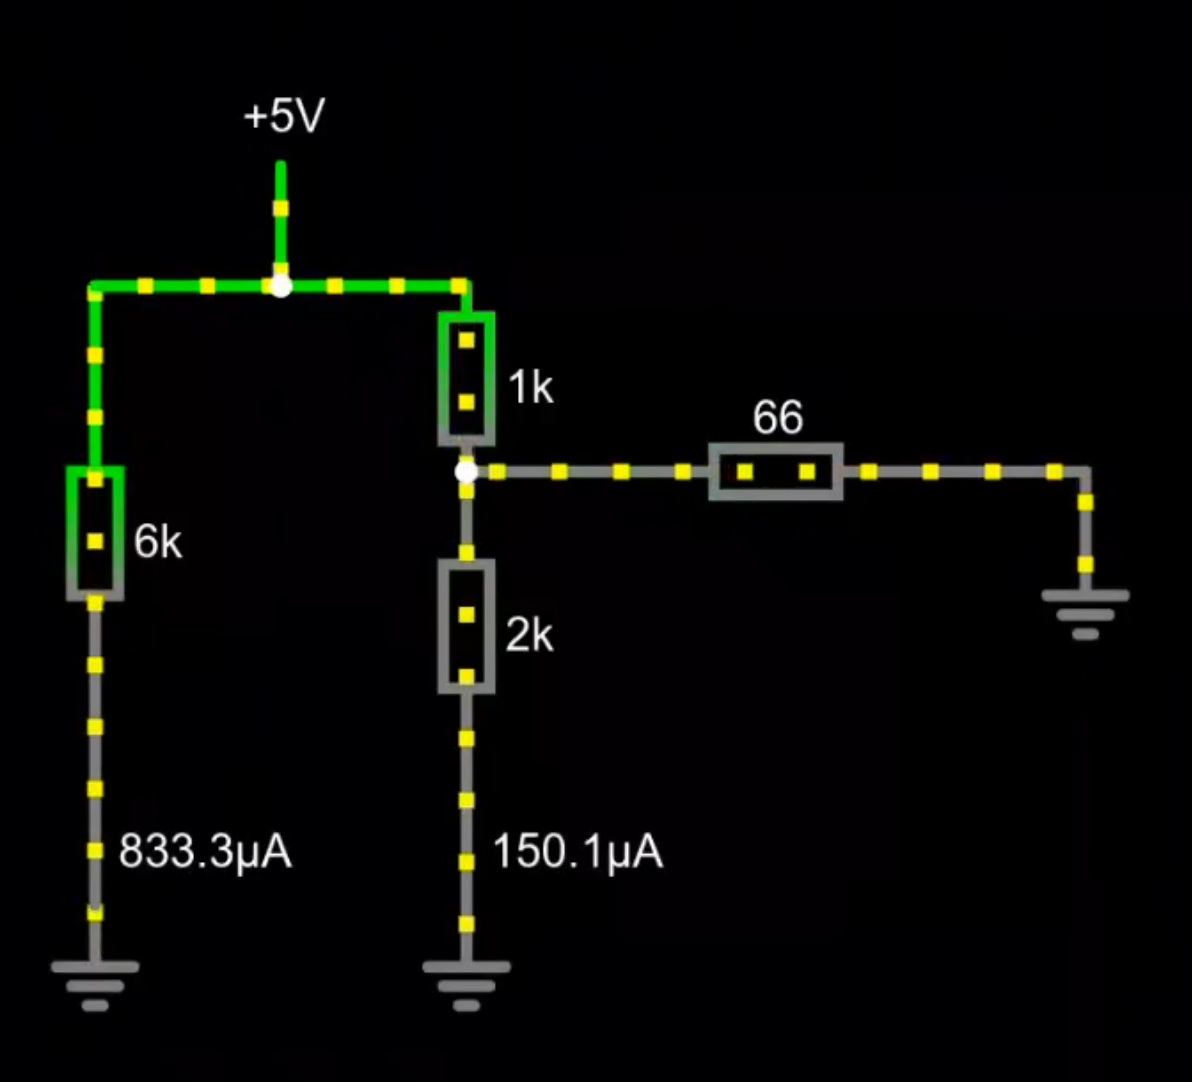
\includegraphics[width=0.25\textwidth]{Images/circuito2.png}
\end{figure}
Il flusso di corrente su suddivide in un ramo e nell'altro. La corrente si distribuisce in maniera proporzionale alla resistenza. Tanto è più bassa, tanto più corrente passa. Per ottenere la resistenza equivalente di due resistenze in parallelo, si usa la formula:
\[ \frac{1}{R_{eq}} = \frac{1}{R_1} + \frac{1}{R_2} \]
\[ R_{eq} = \frac{R_1 \cdot R_2}{R_1 + R_2} \]
\\subsection{Segnale}
Mettere le resistenze in parallelo è utile quando dobbiamo dissipare la potenza.
\\ Qualsiasi carico attacchiamo, esso influisce su tutto il circuito.
\\ Alimentare qualcosa con un partitore non è intelligente. Cosa si può attaccare quindi al partitore disturbandolo il meno possibile? Nell'immagine sopra, estraiamo la potenza dal partitore (molto piccola), invece se modifichiamo la resistenza in parallelo:
\begin{figure}[H]
    \centering
    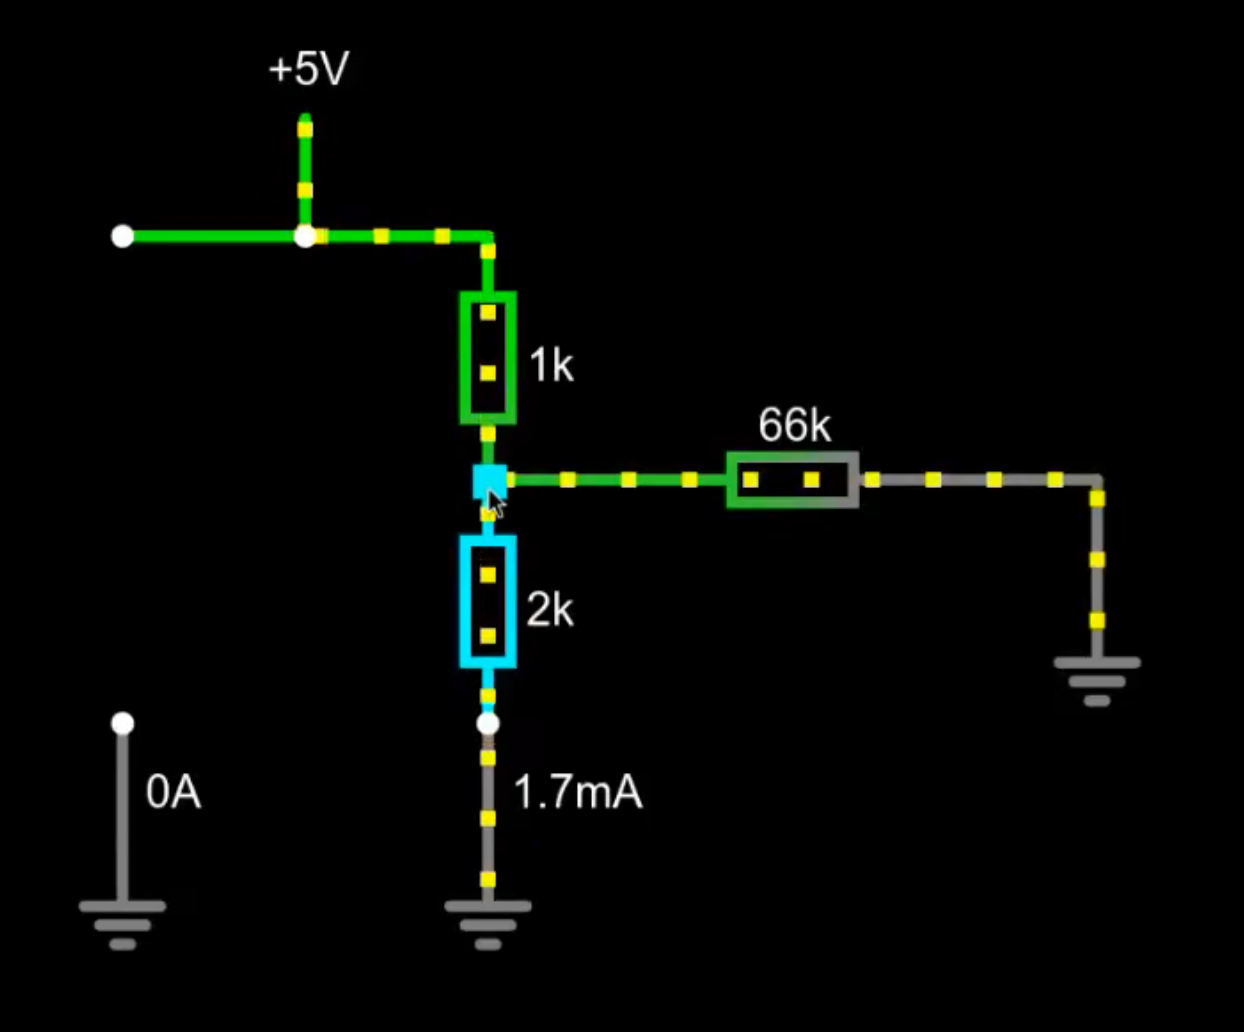
\includegraphics[width=0.25\textwidth]{Images/gpio.png}
\end{figure}
In questo modo, la resistenza in parallelo è molto più grande di quella del partitore, e quindi la corrente che passa è molto più piccola. Viene usato come segnale.
È un carico che influenza poco il partitore, perchè porta via il minimo indispensabile. Esso porta \textbf{informazioni}. Se quella resistenza è un qualche tipo di circuito che memorizza un bit alto se deve passare qualcosa e un bit basso se non deve passare niente, porta informazione.
Porta informazione se nella parte collegata in parallelo c'è tensione o meno. Non si sa che tensione c'è, ma si sa solo che c'è una tensione sufficiente a far dire che sta passando la corrente. La quantità di corrente da dare per scrivere dipende dal tipo di circuito.
\\ Si può calcolare la resistenza interna del gpio. Il gpio si può considerare come una resistenza. Il GPIO lo usiamo in output e input. Se uso il GPIO per leggere un dato bisogna confranotarsi con la circuiteria che c'è intorno. Se lo uso come "interruttore", lo si mette in serie al circuito. Bisogna fare attenzione
però alla resistenza perchè ha un resistenza bassa ma dissipazione massima. Si comporta come una resistenza di basso valore, ma non di grande potenza. Se usiamo quindi il GPIO come sinc per una cosa di qualche ampere si brucia, perchè lì può passare solo qualche decina di milliampere.
\\ Un GPIO si può utilizzare come
\begin{itemize}
    \item alimentazione;
    \item lettura di uno stato elettrico;
    \item interruttore;
\end{itemize}
\pagebreak
\section{Lezione 6}
Il GPIO è il pin con 3.3 volt. Attenzione ad attaccare i poli giusti nei led, il lato lungo, l'\textbf{anodo}, è il polo positivo, mentre l'altro il \textbf{catodo} è quello negativo.
\\ Nelle specifiche di un oggetto è indicata in quale condizioni il dispositivo funziona. Non è solo quindi la parte elettronica da considerare, ma anche tutti gli aspetti esterni.
\\ Il GPIO da al massimo 20 mA.
\\ Nel setup, dobbiamo indicare quale pin vogliamo programmare e come deve funzionare. Ad esempio, se ho collegato sul pin 13 un led, devo indicare che il pin in utilizzo è il 13.
\begin{figure}[H]
    \centering
    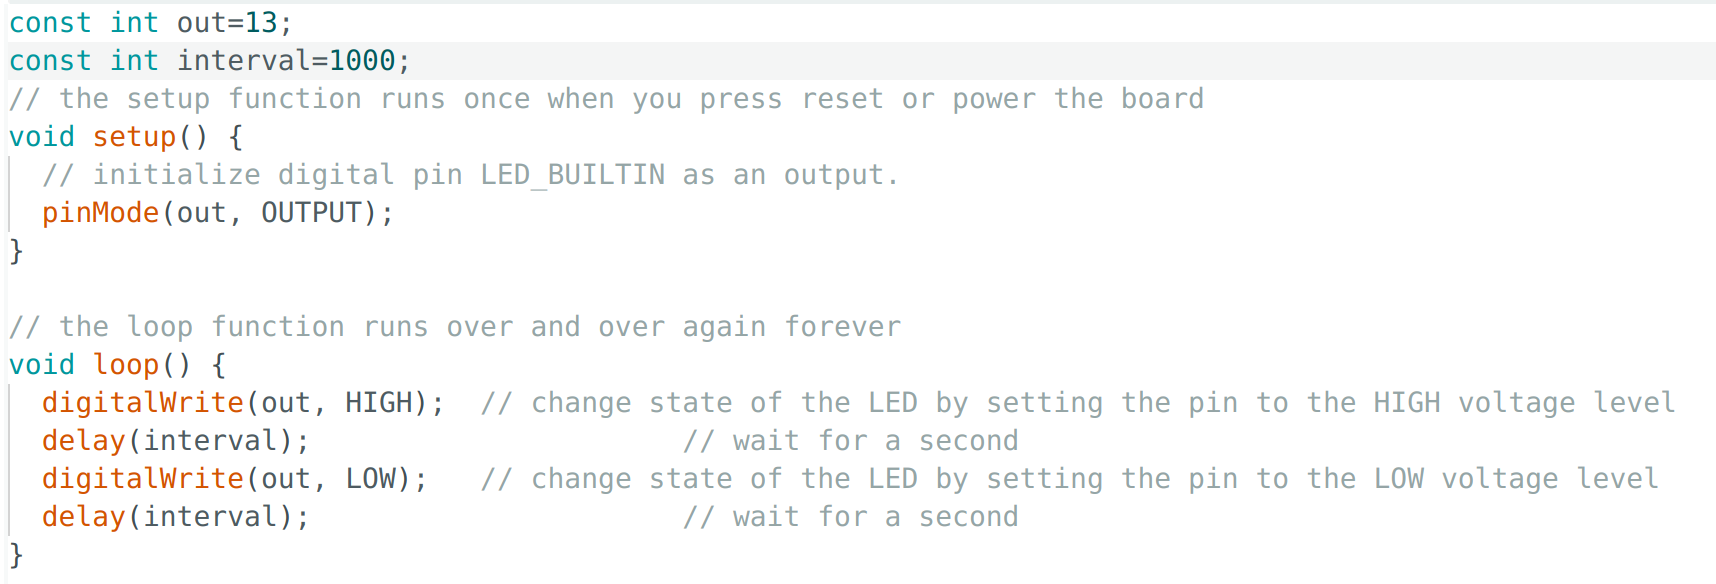
\includegraphics[width=1\textwidth]{Images/blink.png}
\end{figure}
Con la classe \texttt{Serial} è possibile comunicare con il computer. Per inizializzare la comunicazione, nel steup va messo \texttt{Serial.begin(115200)} dove 115200 è la velocità di trasmissione in baudrate.
Per stampare, utilizzo \texttt{Serial.print()}. Posso fare anche l'input, dopo averlo inizializzato nel setup, posso fare \texttt{digitalRead(in)}.
\section{Lezione 7}
\begin{figure}[H]
    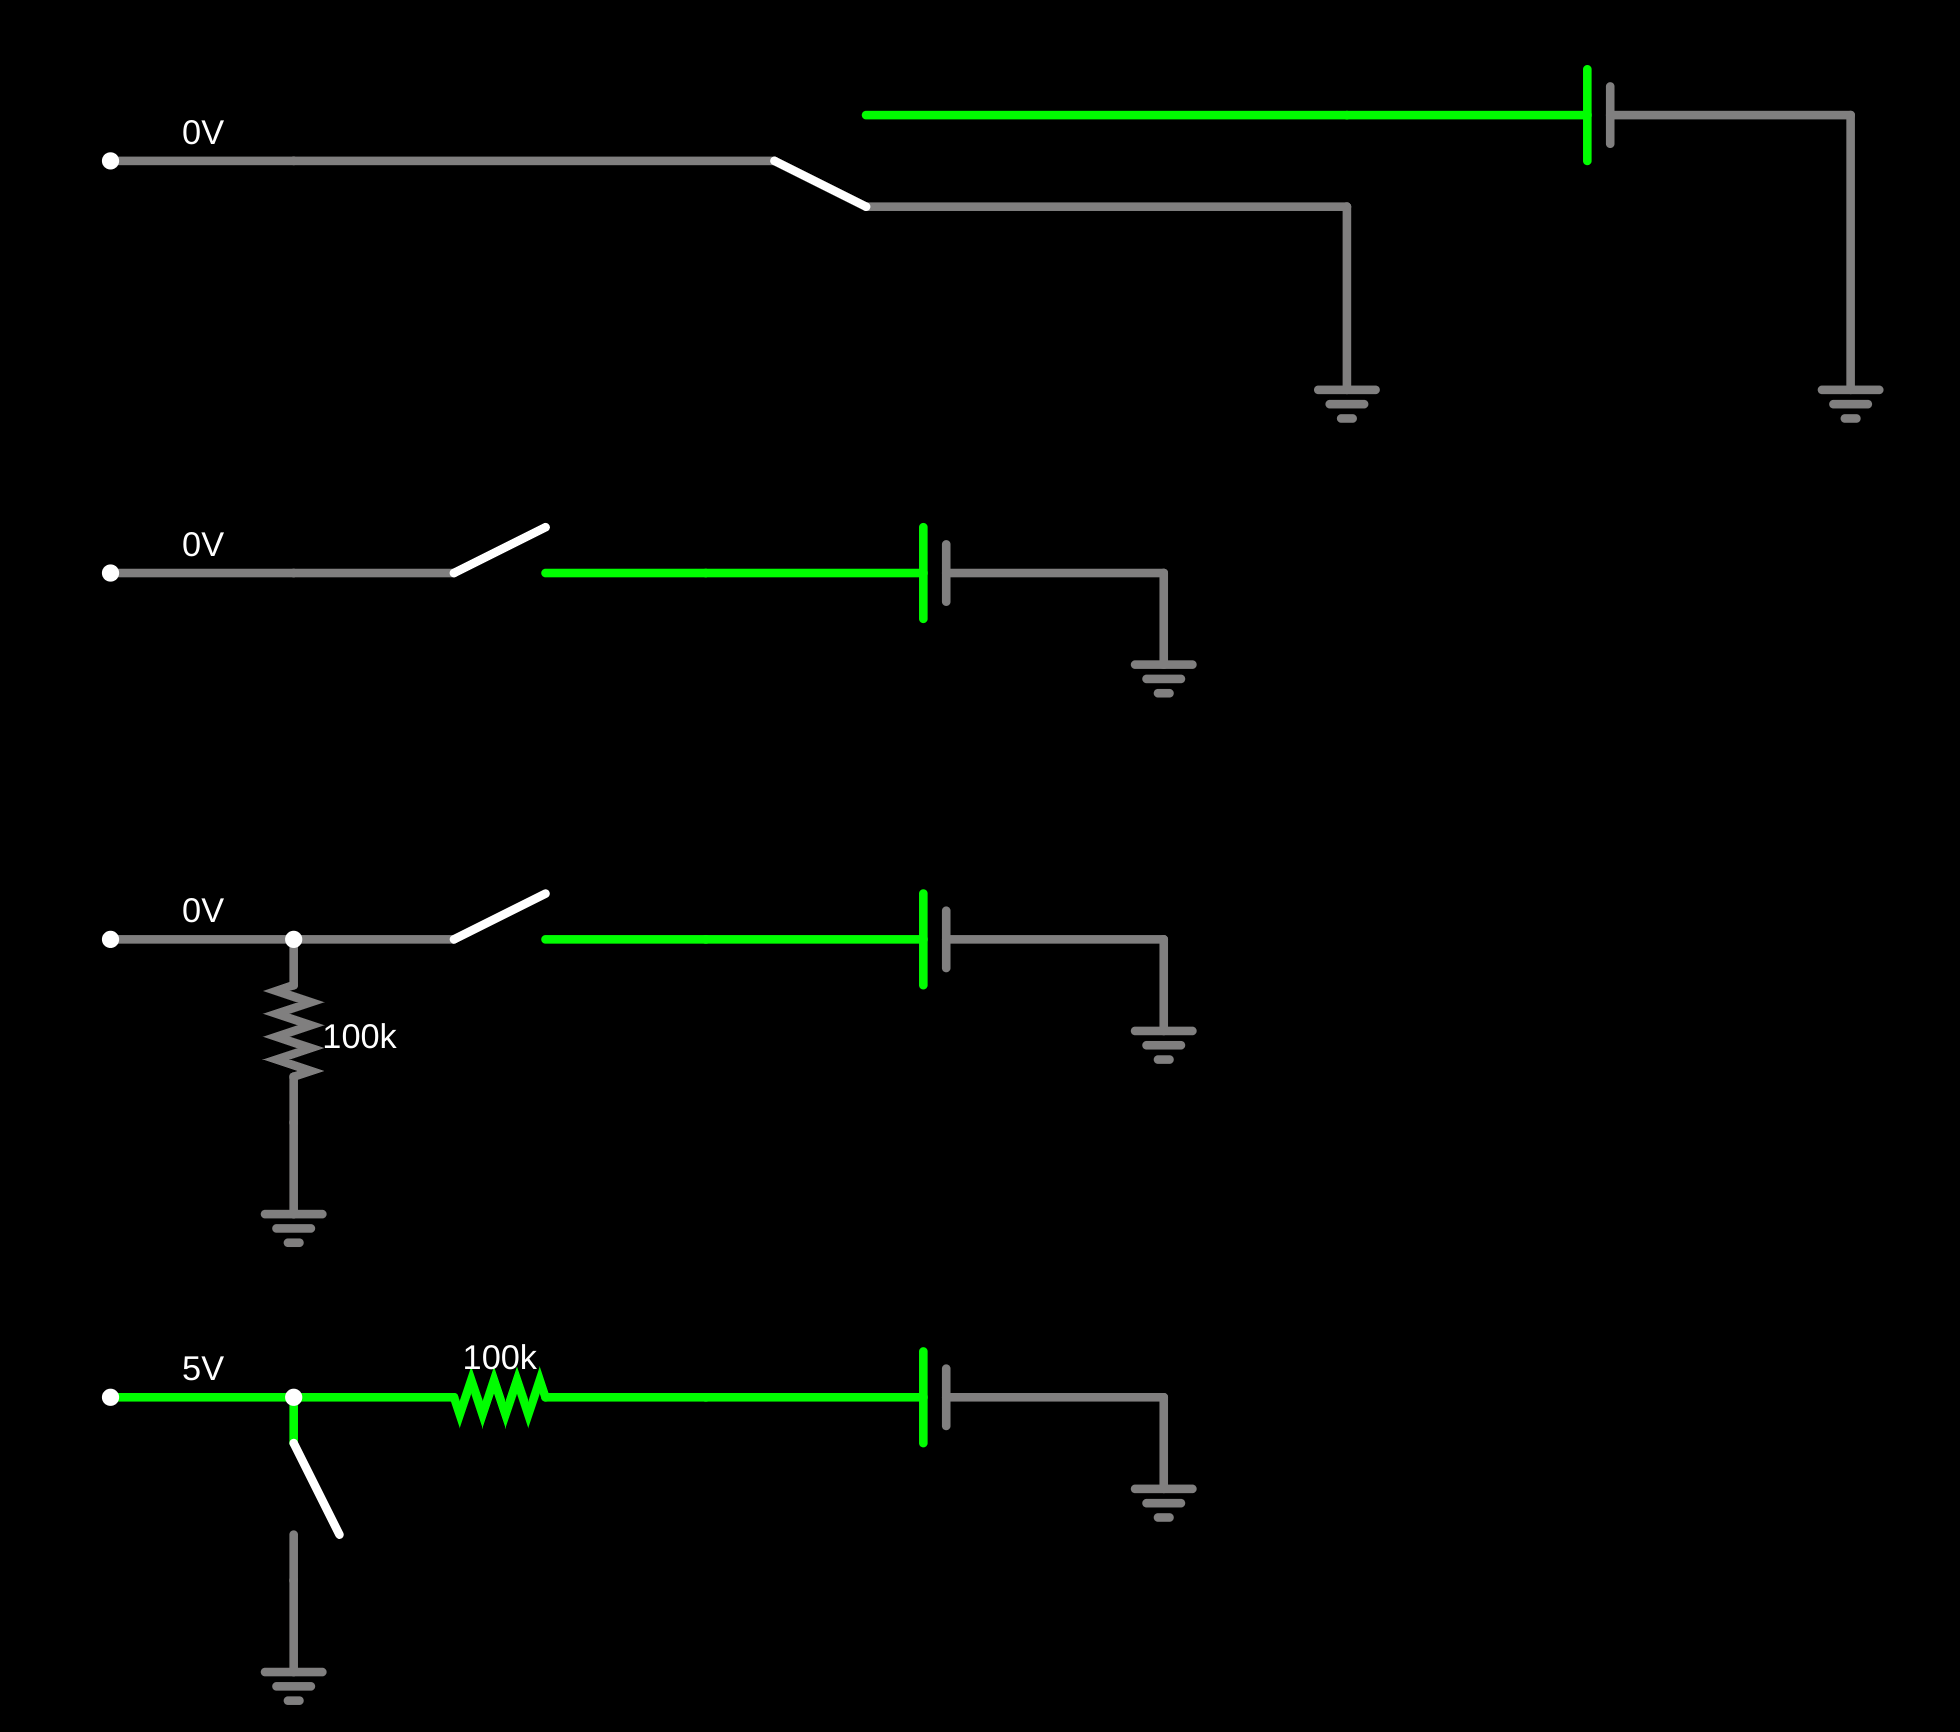
\includegraphics[width=0.5\textwidth]{Images/pullupdown.png}
    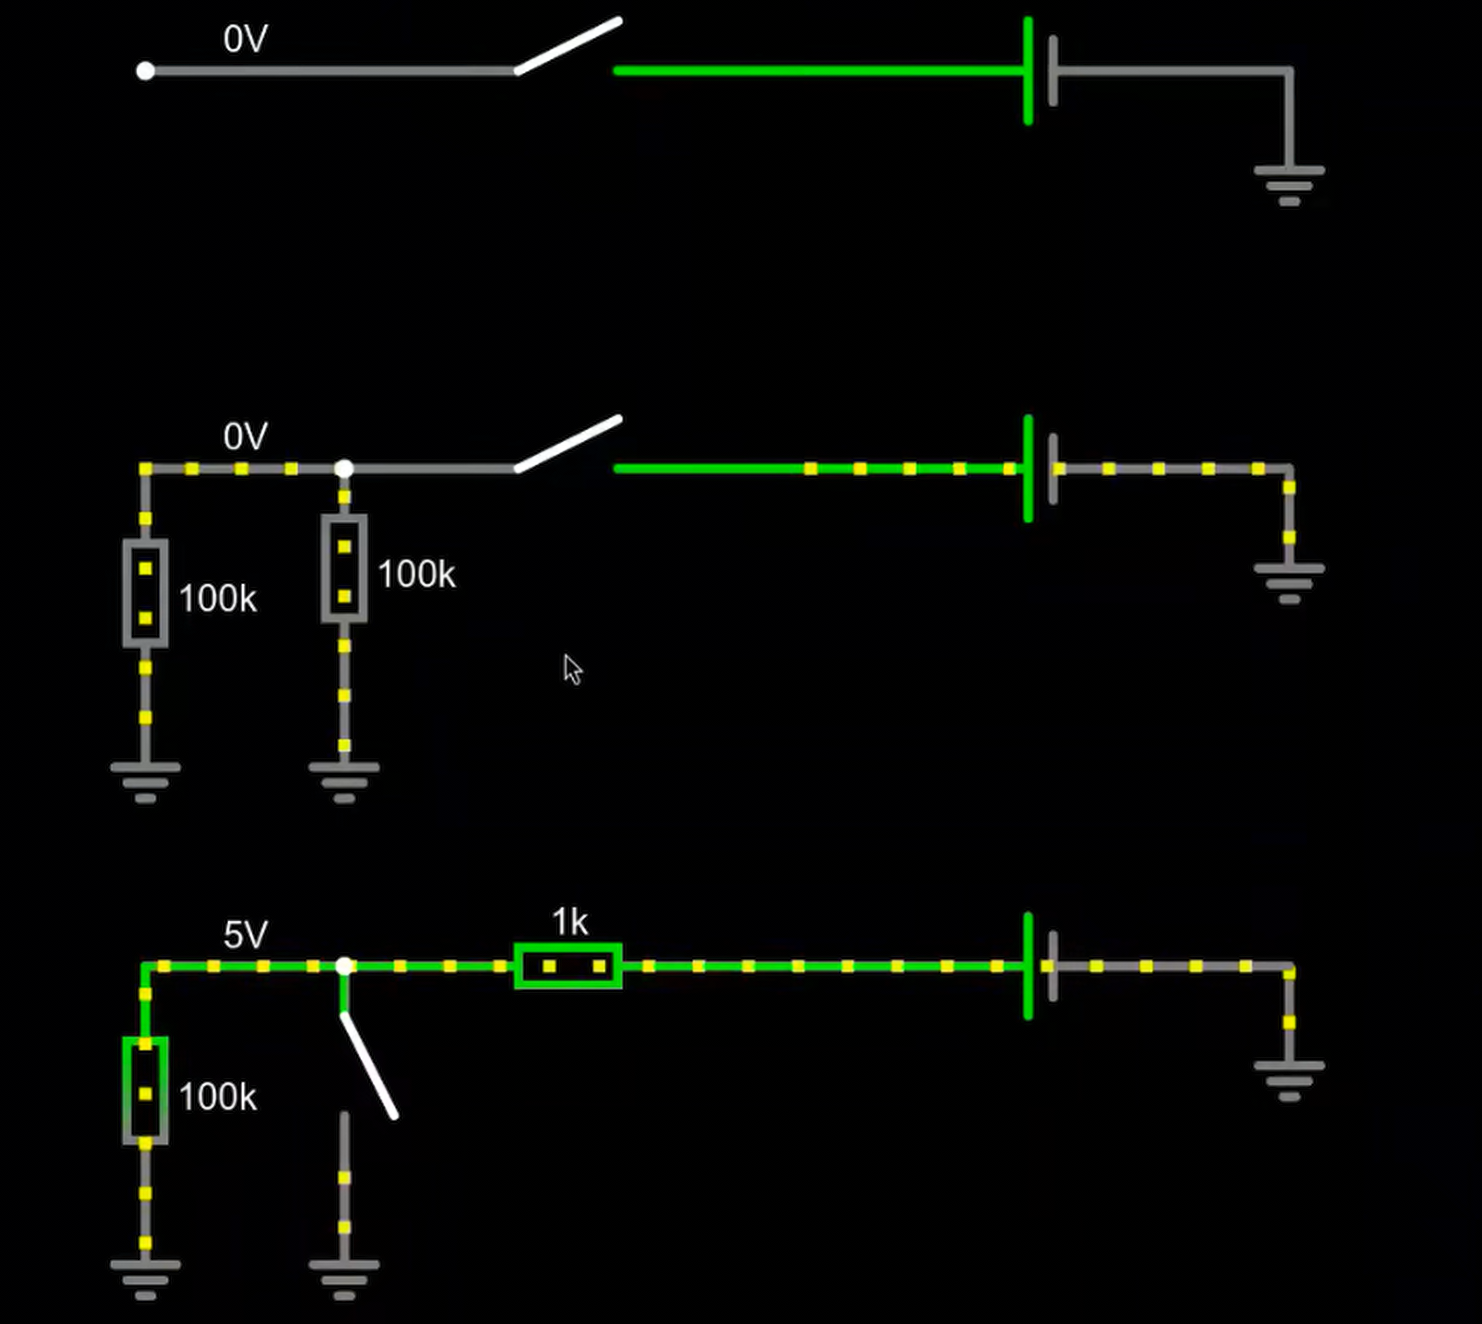
\includegraphics[width=0.5\textwidth]{Images/pullupdown2.png}

\end{figure}
Il \textbf{bottone} o interrope o chiude il circuito, mentre il deviatore non interrompe/chiude, ma semplicemente chiude 2 circuiti diversi. Il bottone quando lo schiaccio cambia stato e quando lo lascio torna allo stato precedente. C'è la distinzione tra \textbf{normalmente aperto} e \textbf{normalmente chiuso}. Nel primo caso,
quando non è premuto, il circuito è aperto, mentre nel secondo caso, quando non è premuto, il circuito è chiuso.
\\ Nell'immagine, normalmente il primo bottone non si usa.
\\ Il terzo è il \textbf{pullup}, quando chiudo il circuito porto giù la tensione. La resistenza di pullup è quella che mi tiene la tensione del GPIO alta, a meno che io non cortocircuiti verso massa.
\\ Ragionando sui valori delle resistenze, la resistenza di pullup deve essere abbastanza bassa in modo che la tensione sia nei limiti \textbf{low} (0-0.8 V) e \textbf{high} (2.8-5 V), la via di mezzo non è determinato, se legge quello, non da informazione.
\\ Nel pinMode, tra le mode c'è l'\texttt{INPUT\_PULLUP} che è il modo in cui dico alla board di attivare il 3 circuito, cioè un meccanismo per cui il gpio internamente ha la resistenza di pullup, attaccat già all'alimentazione. A noi interessa solo attaccarci un bottone che va a massa.
\\ Quando si chiude il circuito, durante la chiusura non c'è un singolo evento. Quindi mentre si chiude, si può leggere 01010101 (\textbf{bouncing}) e quindi magari, nel momento in cui andiamo a leggere, leggiamo uno dei valori di passaggio, dando così una interpretazione errata. Col GPIO resto in ascolto, leggendo veloccisamnete (polling), in cui quando legge un cambio di valore,
ignora la lettura per un periodo di tempo, verificando così un cambio di stato. Sono certo che il cambio di stato lo è se uso uno dei 2 circuiti 2 o 3. Questa cosa si chiama aperazione di \textbf{debouncing}. La durata del bouncing non la conosciamo, quindi la durata è programmabile (un progetto potrebbe essere la programmazione dinamica con dei sensori). Non mettersi a fare il
debouncing a mano, perchè ci sono librerie già create da altri. Se calcoliamo il tempo troppo piccolo prende gli errori, se è troppo grande non prende i comandi iterattivi. Invece di fare polling, si fa \textbf{interact}, ovvero quando c'è un cambio di stato, esegue una funzione (in cui si farà debouncing).

\subsection{GPIO analogico}
Finora abbiamo parlato di GPIO digitali, ma esistono anche quelli \textbf{analogici}. In quelli digitali, in output o do tensione o metto a massa, mentre in input leggo una tensione. I GPIO analogici (non tutte le board le hanno) permettono di
\begin{itemize}
    \item Conversione AD (analogico-digitale), in input, legge una tensione, la misura e resituisce un numero. La tensione viene misurata usando una resistenza. Bisogna cambiarlo il meno possibile, il che significa che deve portare via la minima corrente possibile. Utilizziamo una resistenza il più alta possibile che porti via quel minimo indispansabile per ottenere una misura.
          C'è una tensione di riferimento (rappresentata da max ranfe) (AREF O VREF sono piedini in cui mettere la tensione di riferimento del comparatore per poi avere la lettura corrispondente) che potrebbe essere la tensione di alimentazione della board o anche qualcosa di diverso. C'è un comparatore che calcola il rapporto tra l'ingresso e la tensione di riferimento e restituisce questa informazione come numero, solitamente intero. Il range max è tipicamente 1024 o 4096. Il numero resituito deve essere
          rapportata. Se misuro 732, ad esempio, 732/1024 * AREF (ad esempio 2V). SE non mettiamo nulla, essi sono collegate all'imentazione, quindi 5V o 3,3V. (aref non può avere tensione superiore all'alimentazione). Perchè scendere? È più preiso, perchè so se devo misurare delle tensioni piccole è inutile lasciarli alte.
          \\ Se ripeto le misure nel tempo.
    \item Conversioen DA (digitale-analogico), in output, fornendo un numero, genera una tensione "programmabile", una tensione tra un minimo e un massimo.
\end{itemize}
Quello analogico genera una tensione programmabile
\section{Lezione 8}
Colleghiamo come il circuito 1, ma funziona come il 3.
\\ Adesso colleghiamo il circuito in pull-up in questo modo:
\begin{figure}[H]
    \centering
    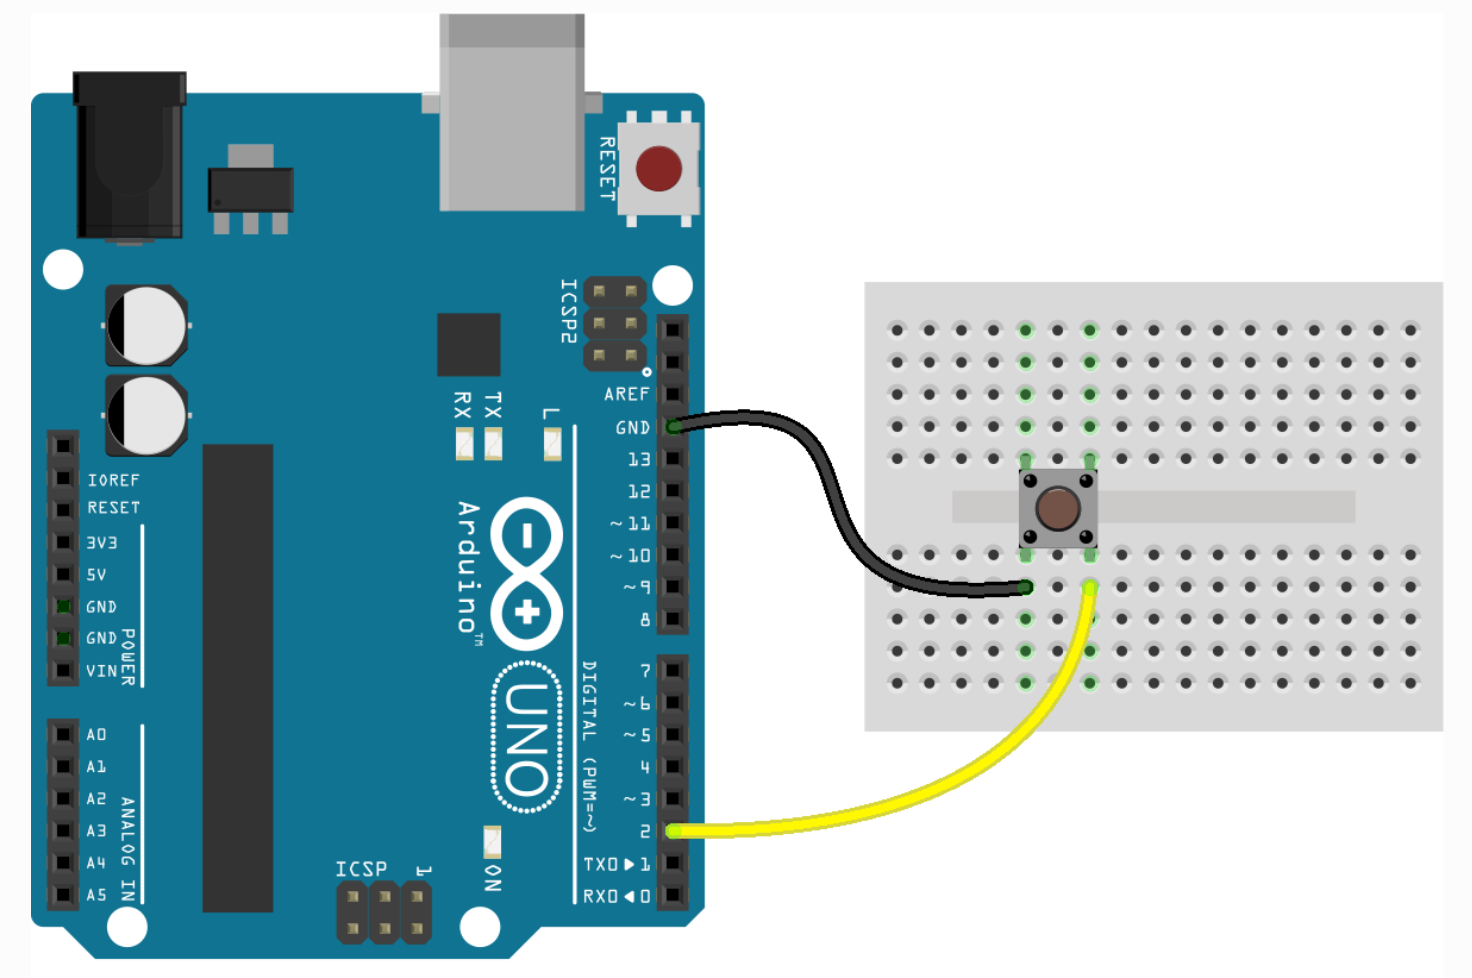
\includegraphics[width=0.5\textwidth]{Images/pullup.png}
\end{figure}
Così facendo, eseguendo questo codice:
\begin{figure}[H]
    \centering
    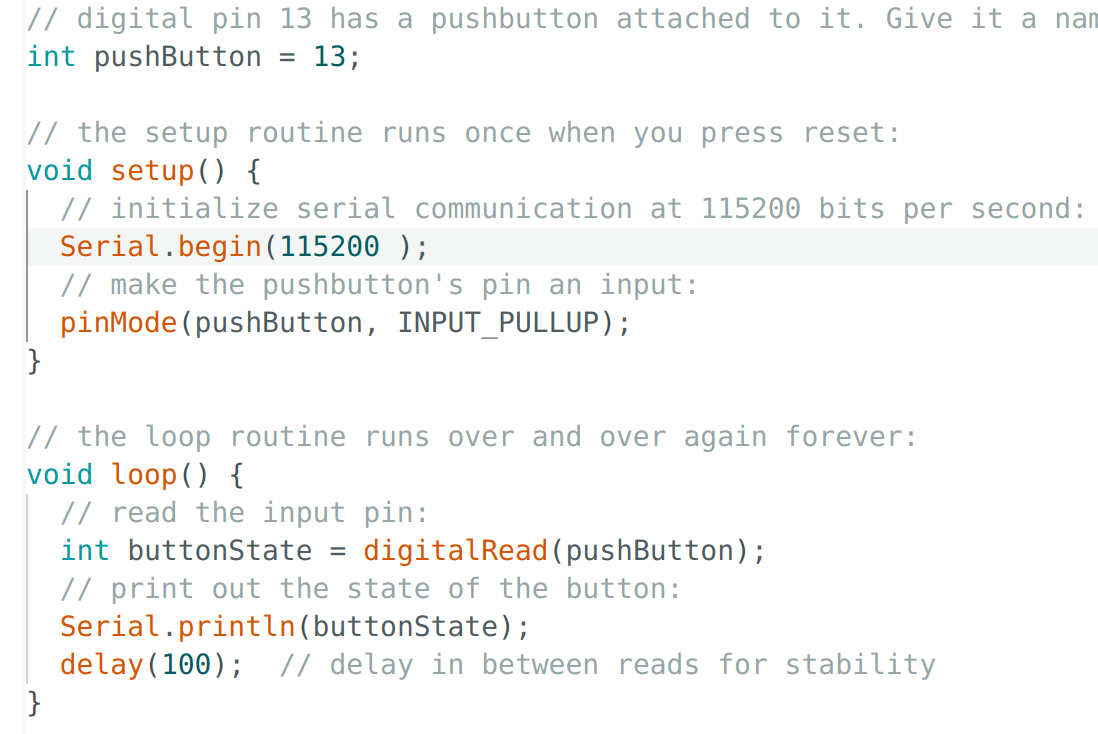
\includegraphics[width=0.5\textwidth]{Images/pullup_code.png}
\end{figure}
Nel monitor si potrà vedere che, a riposo restituisce 1, mentre se clicco il bottone restituisce 0. Utilizzando l'analogico invece, se non premo il bottone, restituisce una serie di numeri, mentre se lo premo, restituisce 0.
\\ Un componente utile sono il \textbf{potenziometro}, che è una resistenza variabile tramite un cursore. I 2 reofori esterni rappresentano il collegamento con la resistenza. Quello in mezzo è il pattino, e fornisce una tensione variabile a seconda della posizione della variabile, quindi:
\begin{center}
    \begin{tabular}{rcl}
        \textbf{Terminale 1} & $\rightarrow$ & GND \\
        \textbf{Cursore}     & $\rightarrow$ & A0  \\
        \textbf{Terminale 2} & $\rightarrow$ & 5V  \\
    \end{tabular}
\end{center}
Un altro componente utile è la \textbf{fotoresistenza}, è un sensore. Possiamo pensare quindi di sostituire il bottone con la fotoresistenza, ma non funziona.
Il circuito corretto è il seguente:
\begin{figure}[H]
    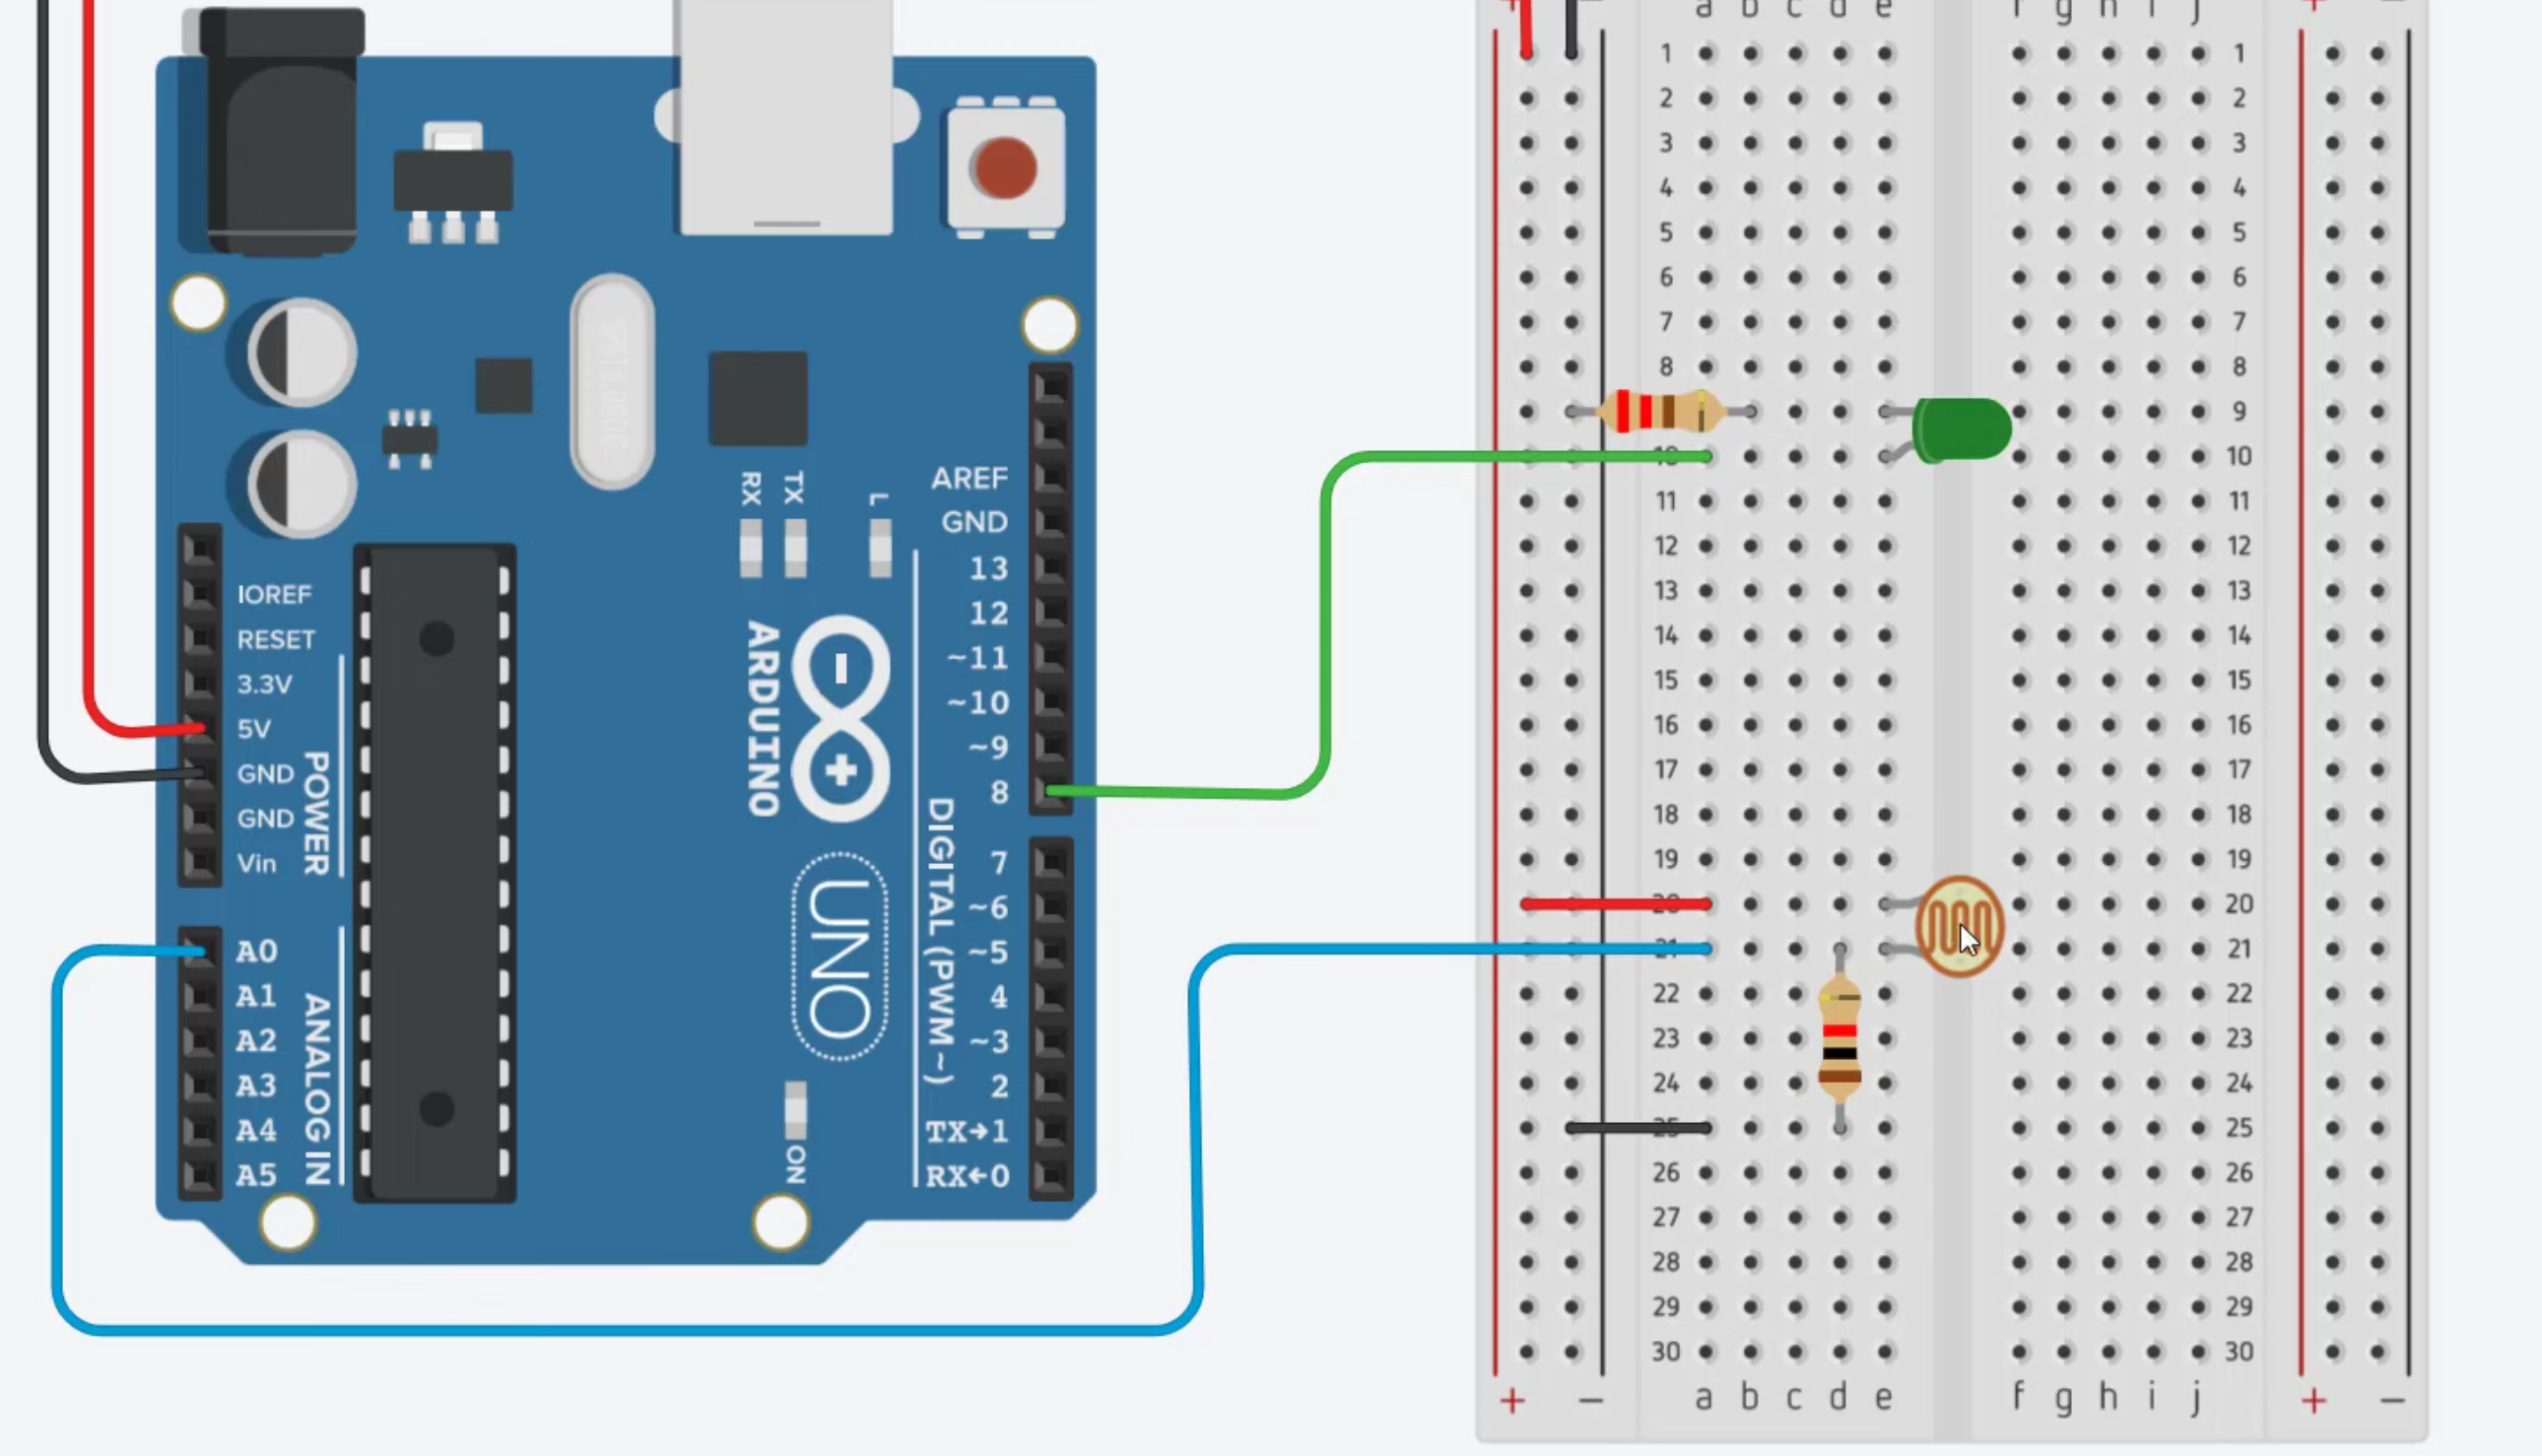
\includegraphics[width=0.5\textwidth]{Images/photoresistor.png}
    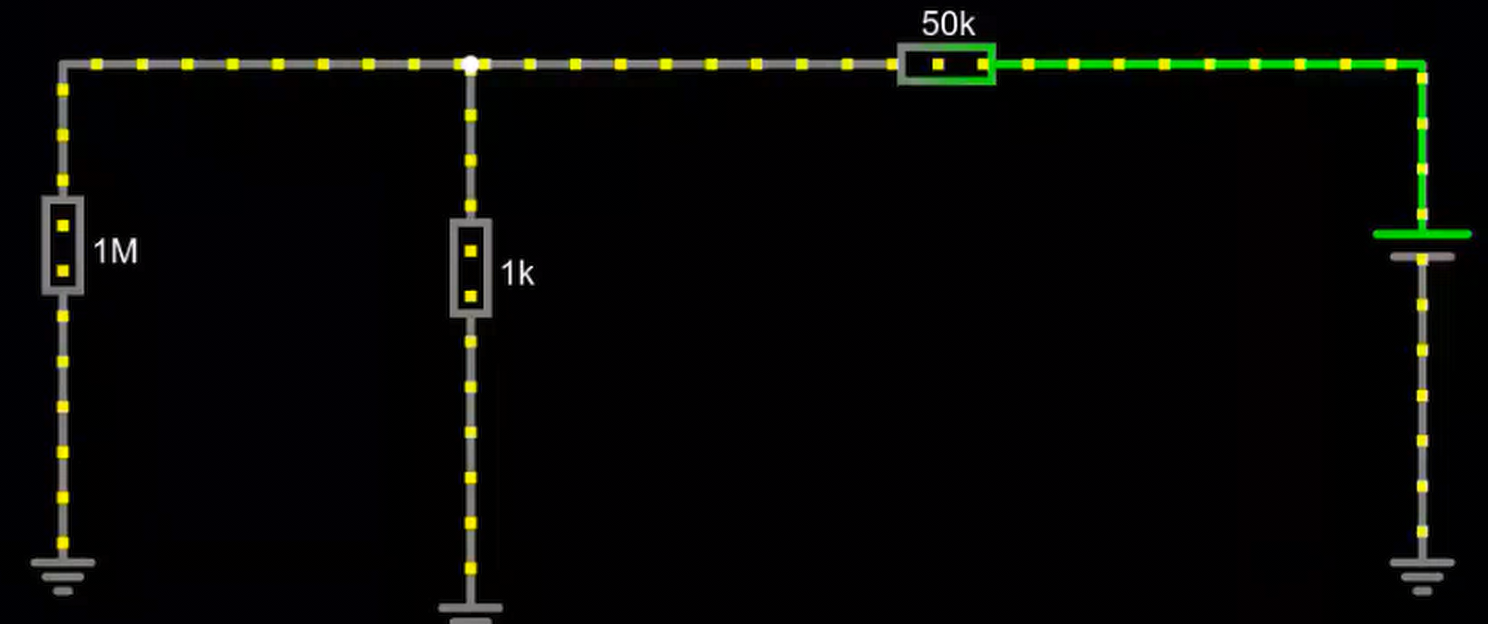
\includegraphics[width=0.5\textwidth]{Images/photoresistor_circuit.png}
\end{figure}
La mia fotoresistenza necessita di una resistenza da 10 Kohm.
\\ Potremmo voler utilizzare un potenziometro al posto della resistenza fissa. Bata quindi sostituirla con il potenziometro:
\begin{figure}[H]
    \centering
    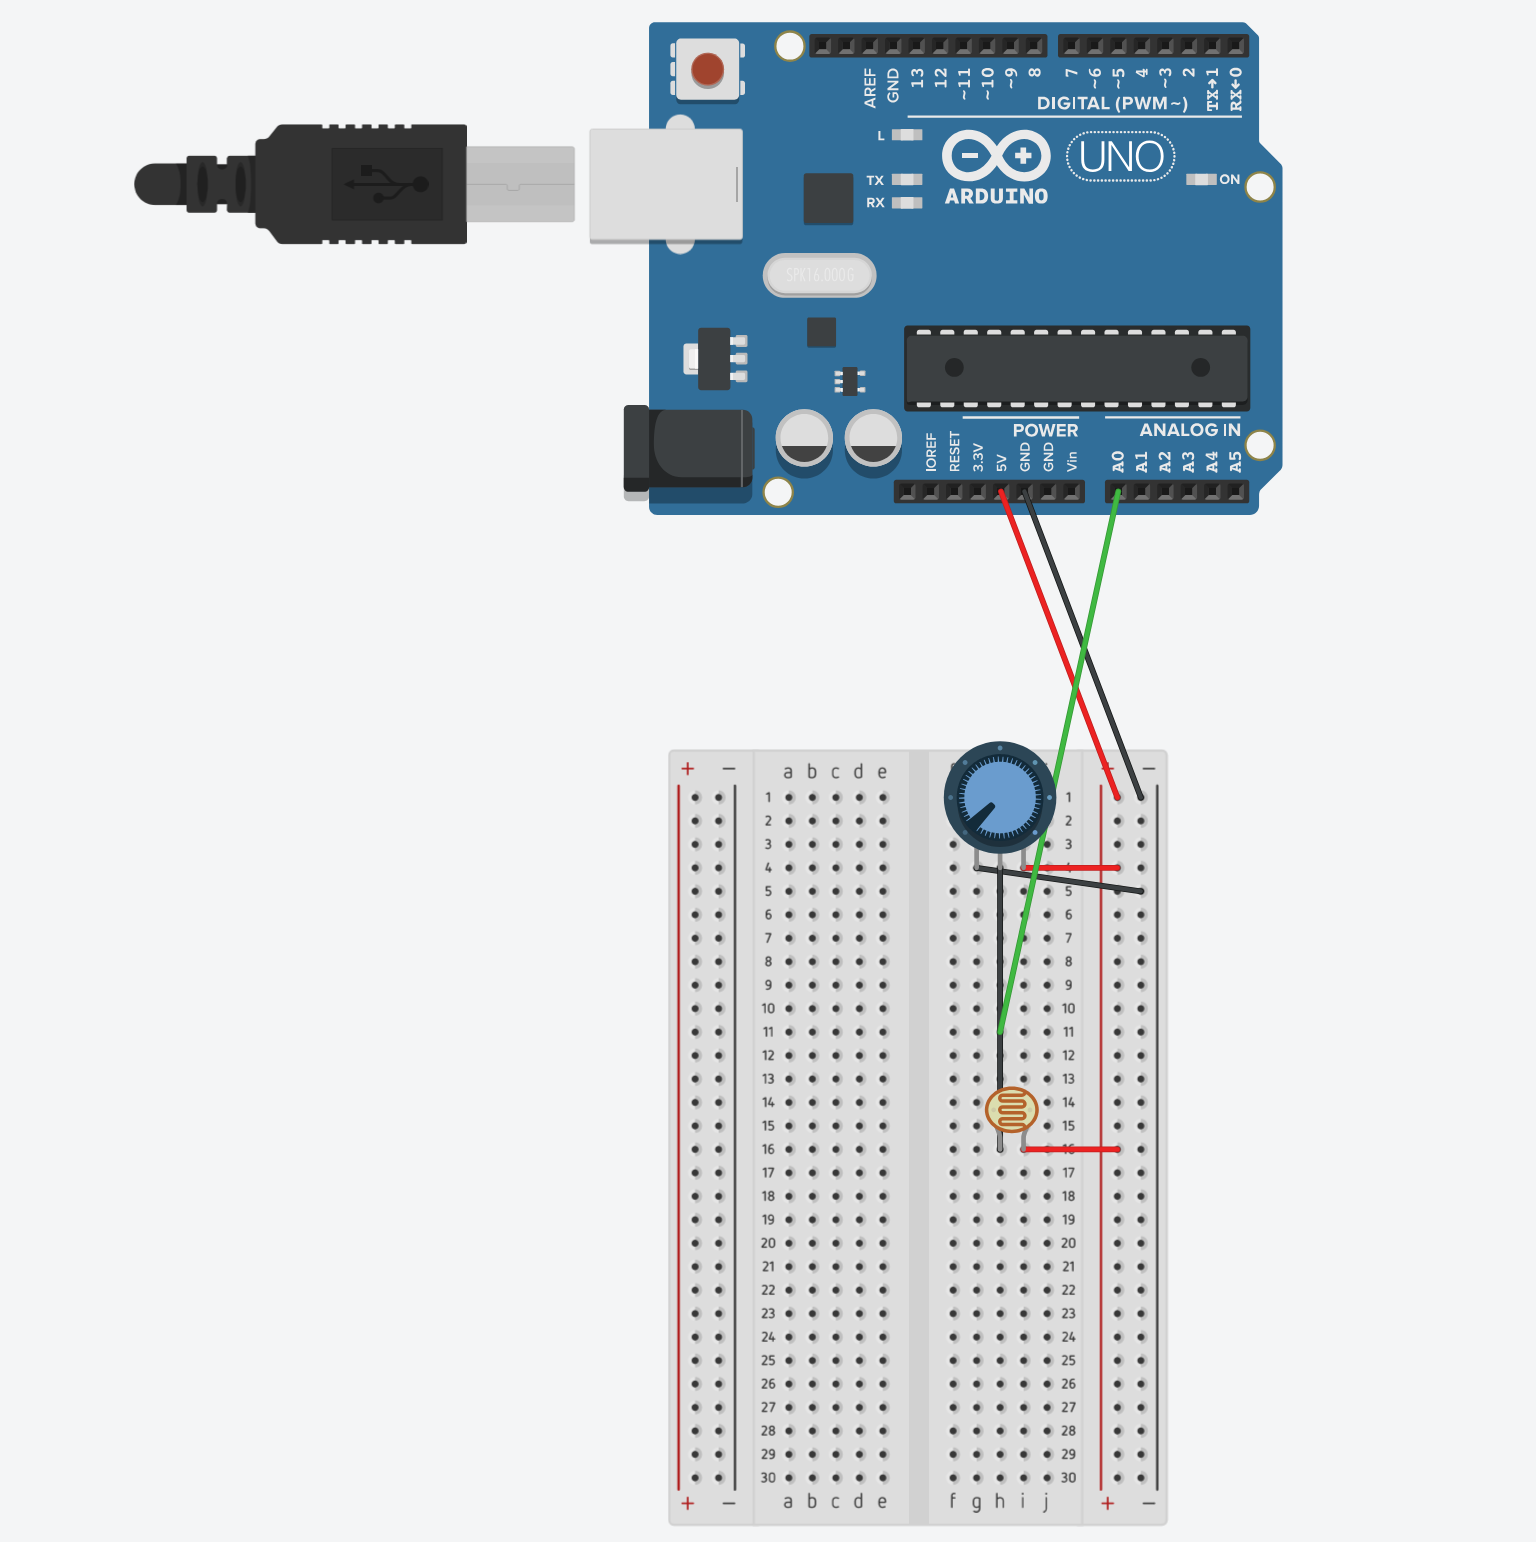
\includegraphics[width=0.4\textwidth]{Images/photoresistor_potentiometer.png}
\end{figure}
Se nel loop voglio campionare nel tempo diversi componenti, ma a tempi diversi, posso usare il metodo \texttt{millis()}. \textbf{NON USARLO, RISCHIO BOCCIATURA}. Se dobbiamo fare cose diverse a periodicità diverse, esistono già delle librerie.
\\ In un progetto reale, nel loop ci troveremo soltanto una singola invocazione di funziona che è la funzione che invocherà poi le altre funzioni.
\\ Perchè vorremmo dare dei temi a diverse funzioni? Perchè magari ci sono funzioni che hanno bisogno di essere eseguite più raramente di altre. Ad esempio, un gps deve essere eseguito meno rispetto ad un rilevamento degli urti. Può essere anche che è il sensore ad essere lento.
\section{Lezione 9}
Il tester quando in modalità tensione usa una resistenza bassa, quando misura l'intensità ha un resistenza bassa.
\\ L'mmetro misura gli ohm di una resistenza. l'ohmetro è un volmetro con un generatore e una resistenza ooportunatametnte collegata. Si misura un singolo componente e questo è il motivo per cui c'è un generatore.
\\ Abbiamo parlato dei GPIO analogici, in cui nell'AREF o VREF si può mettere la tensione di riferimento. Per mettergli la tensione che vogliamo, si utilizza un \textbf{partitore}. È utile metterci 1V quando sappiamo che la variazione di tensione che dobbiamo misurare è giù di lì e quindi è inutile usare i 5 o 3.3 V.
\paragraph{Conversione DA} \mbox{} \\
DA $\Rightarrow$ OUTPUT (fornendo un numero, genera una tensione programmabile "continua"). Non tutte le board hanno il da (la mia la ha in AO). Il codice è \texttt{analogWrite}, in cui si da un numero tra 0 e 255 e il numero del piedino ed emette sul piedino una tensione corrispondente rispetto alla tensione di riferimento.
Serve più che altro per generare un'\textbf{informazione}. Se vogliamo ad esempio alimentare una ventola, essa non parte perchè il GPIO non è in grado di erogare abbastanza corrente (intensità), visto che eroga pochi mA.
\\ Esiste un modo strano di fare un uscita "analogica" usando una tecnica chiamata \textbf{PWM} che non ha bisogno di tutti i componenti di un DAC. Essa è più semplice da realizzare. Se il sistema ha una certa \textbf{inerzia} accendendo e spegnendo con regolarità il circuito di alimetnazione ottengo un effetto fisico che è equivalente ad alimentare
quell'oggetto con una tensione inferiore a quella nominale. Il PWM si basa su questo.
\\\textbf{Duty cycle}: data una PWM, un duty cycle è la percentuale di tempo in cui il segnale è alto. Se il duty cycle è del 50\%, significa che il segnale è alto per metà del tempo e basso per l'altra metà. Se il duty cycle è del 100\%, significa che il segnale è sempre alto, mentre se è del 0\%, significa che il segnale è sempre basso.
\\ \textbf{Tensione efficace}: è la tensione equivalente continua che potrei utilizzare. È l'analogo per fare lo stesso lavoro. È la tensione equivalente continua di una tensione che varia nel tempo.
\\ Cosa ci faccio con un PWM attaccato ad un GPIO? Lo si può utilizzaare con un relè, però non ci piace, perchè fa un suono e poi comunque il relè si consuma. Si utilizza il \textbf{transistor}.
\\ Alla PWM ci posso attaccare un LED, anche se esso non ha inerzia. Assicurarsi che ci sono GPIO con PWM (indicati con \textasciitilde{}). Si usa \texttt{analogWrite(pin, duty\_cycle(0-255))}, lo stesso del DAC. Con il LED, vediamo che in base al valore che diamo alla write, il led diventa più o meno luminoso.
\section{Lezione 10}
\subsection{Interrupt}
Si esegue il polling quando il sensore non è in grado di inviare informazioni. Il che vuol dire chiedergli continuamente lo stato. Non tutte le board supportano l'interrupt
\\ Il meccanismo di comunicazione si basa su un segnale elettrico.
\\ \textbf{ISR}: Interrupt Service Routine. Il programma viene interrotto e viene invocata una funzione che nel momento in cui termina, il programma continua.
\\ Nel setup si prepara l'operazione di reazione, mentre nel loop faccio quello che voglio. \texttt{attachInterrupt(...)}.
ISR è una funzione associata ad un interrupt.
\paragraph{Condizioni} \mbox{}
\\ Su un determinato piedino digitale posso misurare 0 (low) o 1 (high). Quali sono le condizioni che posso sfruttare questo meccanismo? Potrebbe essere high, low oppure la transizione. Le transizioni da low ad high si chiama \textbf{raising}, contrario \textbf{falling}. Un'altra condizione è \textbf{changing} cioè una condizione che dice che non importa quale dei due è, basta che ho una cambiamento.
\\ Notare la presenza dei tempi di risposta di un interrupt caratteristico ad ogni board.
Per disabilitare gli interrupt, si usa \texttt{noInterrupts()}, mentre per riattivarle \texttt{interrupts()}.
\paragraph{Funzione ISR} \mbox{}
\\ La funzione ISR deve essere \textbf{breve} perchè se la board è sorda agli altri interrupt durante il service di quell'interrupt, se facciamo una cosa lunga gli altri interrupt non vengono ascoltati. Non ha parametri di ingresso e di ritorno e meglio non chiamare altre funzioni "pesanti" (tipo \texttt{Serial.print()}).
\\ Non tutte le board supportano gli high x.
\\ Attenzione al bouncing. IRAM\_ATTR dice al compilatore di allocare la funzione nel posto "giusto" (ovvero nella memoria più veloce).
\section{Lezione 11}
\subsection{Componenti}
\subsubsection{Interruttore}
Un interruttore interrompe il flusso di corrente a comando.
Il relè è un interruttore controllato elettricamente.
\subsubsection{Lampadine}
\subsubsection{Relè}
Il relè è un interruttore controllato elettricamente.
\begin{figure}[H]
    \centering
    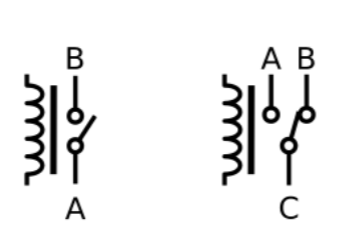
\includegraphics[width=0.25\textwidth]{Images/relè.png}
\end{figure}
La bobina fa parte di un circuito, mentre l'altro è un altro circuito.
\subsubsection{Condensatore}
Una delle applicazioni del condensatore è quella di fare debouncing: è possibile mettere un condensatore opportunatamente ad un bottone per ridurre il debouncing.
\\ La tensione del condensatore non supera mai quella di alimentazione, ma si carica lentamente.
\\ I condensatori con isolante elettrolitico hanno una polarità, quindi bisogna fare attenzione perchè se li attacchiamo al contrario, esplodono.
\subsubsection{Semiconduttori}
\section{Lezione 12}
\subsubsection{Sensori (quelli rossi)}
\begin{figure}[H]
    \centering
    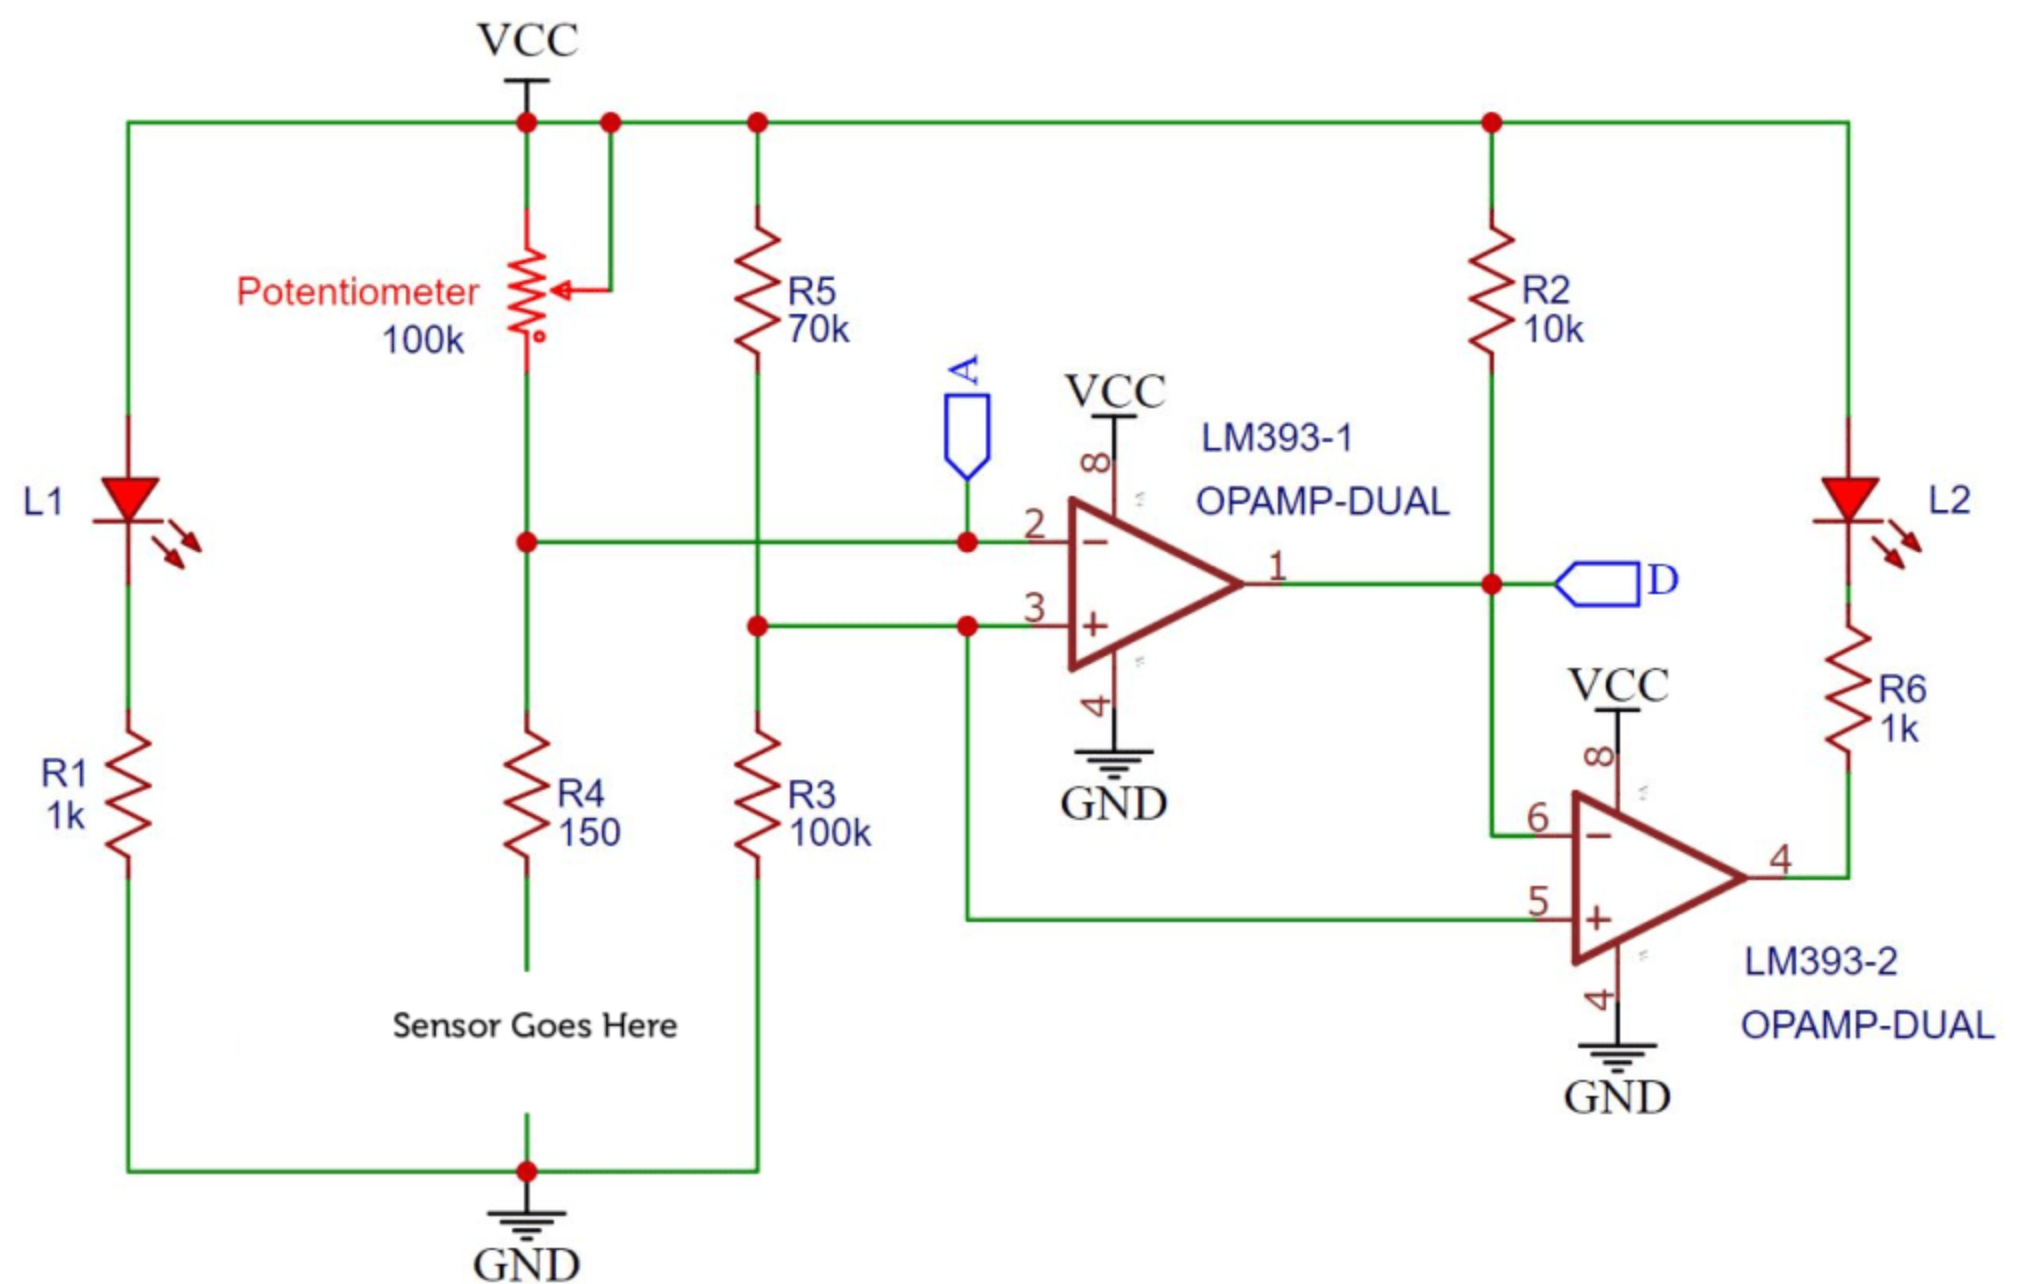
\includegraphics[width=0.5\textwidth]{Images/circuito3.png}
\end{figure}
Il componente triangolare è un \textbf{amplificatore operazionale}, amplifica il segnale che arriva in ingresso in uscita. I due ingressi servono a "sommare" i due segnali.
Li somma prendendo il segnale con il + (non invertente) e lo ribalta in caso di quello invertente.
\\ La linea 2 è collegata ad un sensore, la 3 è invece collegata all'imentazione con un partitore. Il potenziometro è collegato in maniera strana: collegato così il partitore diventa una resistenza variabile: il cursore cortocircuita fino ad un certo punto.
\subsection{Tasking}
\paragraph{Process} \mbox{}: SO, mem dedicata (MMU), gerarchie, risorse
\paragraph{Task} \mbox{}: funzione, no SO, mem condivisa.
\paragraph{Thread (fisico)} \mbox{}: "contesto" di esecuzione (PC, SP, etc).
\paragraph{Cooperative} \mbox{}: se io thread fisico sto eseguendo una certa funzione, se lo sto eseguendo non c'è niente che mi fa cambiare idea.
\paragraph{Preemptive} \mbox{}: se ho un sistema preemptive è possibile essere interrotto, interrupt.
\subsubsection{Cooperative}
Il cooperative semplice non ammette interruzioni. Esiste il cooperative con yield in cui un task può decidere di cedere il controllo ad un altro thread, ma è sempre lui a decidere quando farlo.
\paragraph{Multithread} \mbox{} (monocore, preemptive): se ho un sistema preemptive, è possibile essere interrotto, interrupt. Il sistema operativo decide quando interrompere un thread e farne eseguire un altro. Il sistema operativo decide quando interrompere un thread e farne eseguire un altro.
\paragraph{Multithread} \mbox{} (multicore): se ho un sistema multicore, è possibile eseguire più task contemporaneamente, senza bisogno di interrompere un thread per farne eseguire un altro. Il sistema operativo decide quando assegnare un thread ad un core e quando spostarlo da un core all'altro.
\\ Vedi codice \href{run:../codice/Tasking/Tasking.ino}{Tasking.ino}. Utilizziamo la libreria \texttt{TaskScheduler}
Il controllo lo diamo completamente allo scheduler nel loop.
\\ Per un buon progetto pensare a \textbf{task}. Servono i prototipi delle funzioni.
\end{document}